%%%%%%%%%%%%%%%%%%%%%%%%%%%%%%%%%%%%%%%%%
% Programming/Coding Assignment
% LaTeX Template
%
% This template has been downloaded from:
% http://www.latextemplates.com
%
% Original author:
% Ted Pavlic (http://www.tedpavlic.com)
%
% Note:
% The \lipsum[#] commands throughout this template generate dummy text
% to fill the template out. These commands should all be removed when
% writing assignment content.
%
% This template uses a Perl script as an example snippet of code, most other
% languages are also usable. Configure them in the "CODE INCLUSION
% CONFIGURATION" section.
%
%%%%%%%%%%%%%%%%%%%%%%%%%%%%%%%%%%%%%%%%%

%----------------------------------------------------------------------------------------
% PACKAGES AND OTHER DOCUMENT CONFIGURATIONS
%----------------------------------------------------------------------------------------

\documentclass{scrartcl}

\usepackage[T1]{fontenc}
\usepackage[utf8x]{inputenc}

\usepackage{fancyhdr} % Required for custom headers
\usepackage{lastpage} % Required to determine the last page for the footer
\usepackage{extramarks} % Required for headers and footers
\usepackage[usenames,dvipsnames]{color} % Required for custom colors
\usepackage{graphicx} % Required to insert images
\usepackage{listings} % Required for insertion of code
\usepackage{courier} % Required for the courier font

\usepackage{hyperref}

\linespread{1.1} % Line spacing

% Set up the header and footer
\pagestyle{fancy}
\lhead{\hmwkAuthorName \\} % Top left header
\chead{\hmwkClass: \hmwkTitle} % Top center head
\rhead{\firstxmark} % Top right header
\lfoot{\lastxmark} % Bottom left footer
\cfoot{} % Bottom center footer
\rfoot{Page\ \thepage\ of\ \protect\pageref{LastPage}} % Bottom right footer
\renewcommand\headrulewidth{0.4pt} % Size of the header rule
\renewcommand\footrulewidth{0.4pt} % Size of the footer rule

\setlength\parindent{0pt} % Removes all indentation from paragraphs

%----------------------------------------------------------------------------------------
%	CODE LISTINGS SETUP
%----------------------------------------------------------------------------------------
\usepackage{color}
\usepackage[usenames,dvipsnames,svgnames,table]{xcolor}
\colorlet{MAROON}{Maroon}
\usepackage{minted}
\providecommand*{\listingautorefname}{Listing}

%----------------------------------------------------------------------------------------
% NAME AND CLASS SECTION
%----------------------------------------------------------------------------------------

\newcommand{\hmwkTitle}{Project 2 -- Building a General Constraint-Based Puzzle Solver} % Assignment title
\newcommand{\hmwkDueDate}{Wednesday,\ October\ 24,\ 2013} % Due date
\newcommand{\hmwkClass}{IT3105} % Course/class
\newcommand{\hmwkClassTime}{} % Class/lecture time
\newcommand{\hmwkClassInstructor}{Lecturer: Keith Downing} % Teacher/lecturer
\newcommand{\hmwkAuthorName}{Pablo Liste Garcia \& Dominik Horb} % Your name


\usepackage{tabularx}
%----------------------------------------------------------------------------------------
% TITLE PAGE
%----------------------------------------------------------------------------------------

\title{
\vspace{2in}
\textmd{\textbf{\hmwkClass:\ \hmwkTitle}}\\
\normalsize\vspace{0.1in}\small{Due\ on\ \hmwkDueDate}\\
\vspace{0.1in}\large{\textit{\hmwkClassInstructor\ \hmwkClassTime}}
\vspace{3in}
}

\author{\textbf{\hmwkAuthorName}}
\date{} % Insert date here if you want it to appear below your name

%----------------------------------------------------------------------------------------

\begin{document}

\maketitle

%----------------------------------------------------------------------------------------
% TABLE OF CONTENTS
%----------------------------------------------------------------------------------------

%\setcounter{tocdepth}{1} % Uncomment this line if you don't want subsections listed in the ToC

\newpage
\tableofcontents
\newpage

\section{Architecture Description}

The general structure we chose to use for our implementation of the general puzzle solver doesn't deviate much from the proposed architecture in the task description. \autoref{fig:architecture} shows the two most important packages we created and their contained types. As you can see the main additions we made are \textit{PuzzleState}, \textit{Conflict} and \textit{GeneralPuzzleSolver}.

Our main class that creates the state manager and algorithm objects, initiates the execution and calculates the statistics is \textit{GeneralPuzzleSolver}. It could probably be refactored to separate the different tasks it has a bit more cleanly and distribute the problem specific initialization steps, but this is trivially achievable and wasn't a priority for now. To start an algorithm it creates an object of the desired \textit{LocalStateManager} for the puzzle that should be solved, provides it to an object of the chosen algorithm and starts the algorithm as can be seen in \autoref{lst:starting}.

\begin{listing}[H]
\caption{Combining algorithm and puzzle and starting the search.}
\label{lst:starting}
\begin{minted}[linenos=true]{java}
this.puzzle = this.choosePuzzle();
this.searcher = this.chooseSearchAlgorithm();
this.searcher.setStateManager(this.puzzle);
    
this.numberOfRuns = this.chooseNumberOfRuns();

PuzzleState currentSolution;

for (int i = 0; i < this.numberOfRuns; i++) {
  currentSolution = this.searcher.run();
  currentSolution.display();
}
\end{minted}
\end{listing}

 \begin{figure}[!htbp]
 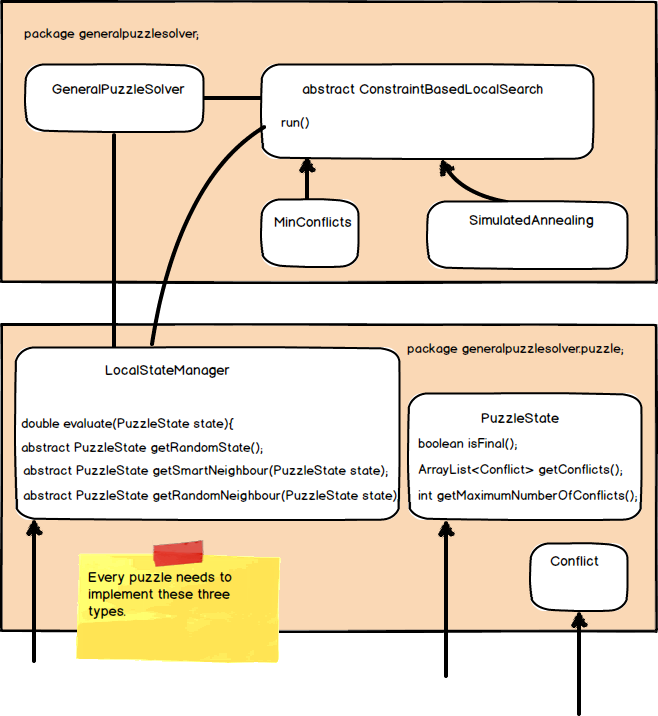
\includegraphics[width=1.0\linewidth]{graphics/architecture-diagram.png}
\caption{Architecture of our general puzzle solver.}\label{fig:architecture}
 \end{figure}

The more important bits can be found in the \textit{generalpuzzlesolver.puzzle} package. All three types that can be seen in the lower part of \autoref{fig:architecture} must be implemented by every puzzle that should be added to the application. The algorithm classes will only interact with methods that can be found within theses three types in order to generalize their execution.

\textit{Conflict} is simply an interface without any methods, but necessary to pass around specific conflicts. For the graph colouring problem an implementation would for example store the indices of two nodes that have the same colour and an edge in the graph.

As the name suggests, an implementation of \textit{PuzzleState} would simply store the data of the current state of the puzzle. It also needs to be able to check if it violates any constraints of the puzzle, provide a list of all the conflicts that exist and display itself.

To provide an example: In case of the graph colouring problem, it contains an adjacency matrix and a list with the data for all the vertices (colour and position).

The \textit{PuzzleStateManager} will be a stateless object in most cases, that just takes \textit{PuzzleState} objects into it's methods and changes them to some kind of ruleset provided inside the method.

\section{First Puzzle: k-Queens}

\begin{table}[!htbp]
\caption{Statistics for the k-Queens puzzle.}
\begin{tabularx}{\textwidth}{l | X | X | X | X | X | X}
Combination & Evaluation  \newline Average & - \newline SD & - \newline Best & Steps \newline Average & - \newline SD & - \newline Lowest \\
\hline
Easy / SA & 0.0 & 0.0 & 0.0 & 76.15 & 52.12 & 8 \\
Medium / SA & 0.0 & 0.0 & 0.0 & 155.70 & 91.20 & 50  \\
Hard / SA & 0.0 & 0.0 & 0.0 & 217.05 & 69.84 & 127  \\
Easy / MC & 0.0 & 0.0 & 0.0 & 218.00 & 211.27 & 7  \\
Medium / MC & 0.0 & 0.0 & 0.0 & 392.55 & 346.81 & 22  \\
Hard / MC & 0.0 & 0.0 & 0.0 & 522.45 & 317.74 & 176  \\
\end{tabularx}
\end{table}

Both algorithms were able to solve the easy case variant of the k-queens puzzle without problems.
The results as shown by our application can be seen in \autoref{fig:queens-sa} for simulated annealing and \autoref{fig:queens-mc} for min-conflicts.

 \begin{figure}[!htbp]
 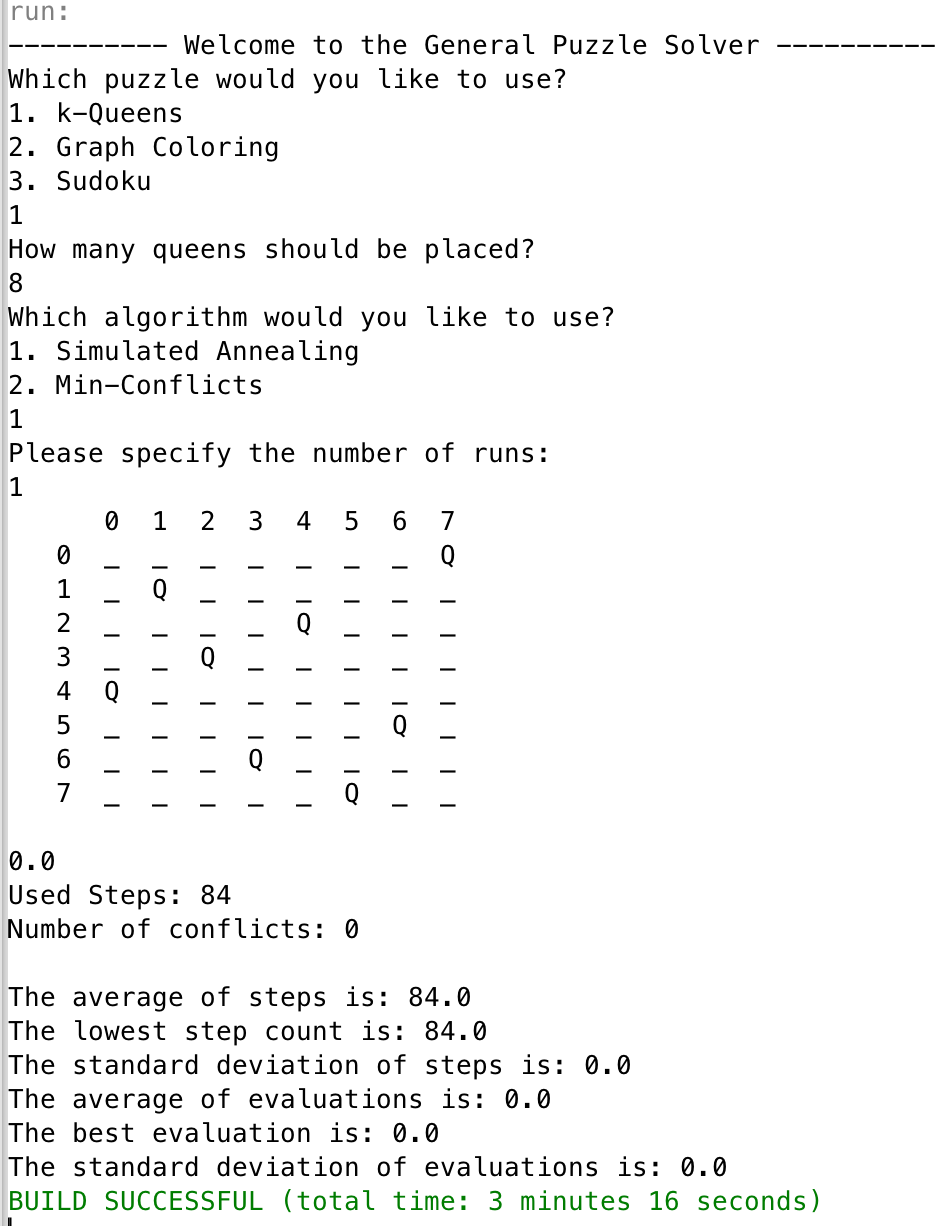
\includegraphics[width=1.0\linewidth]{graphics/queens-sa.png}
\caption{Solution of 8-Queens with simulated annealing.}\label{fig:queens-sa}
 \end{figure}
 
  \begin{figure}[!htbp]
 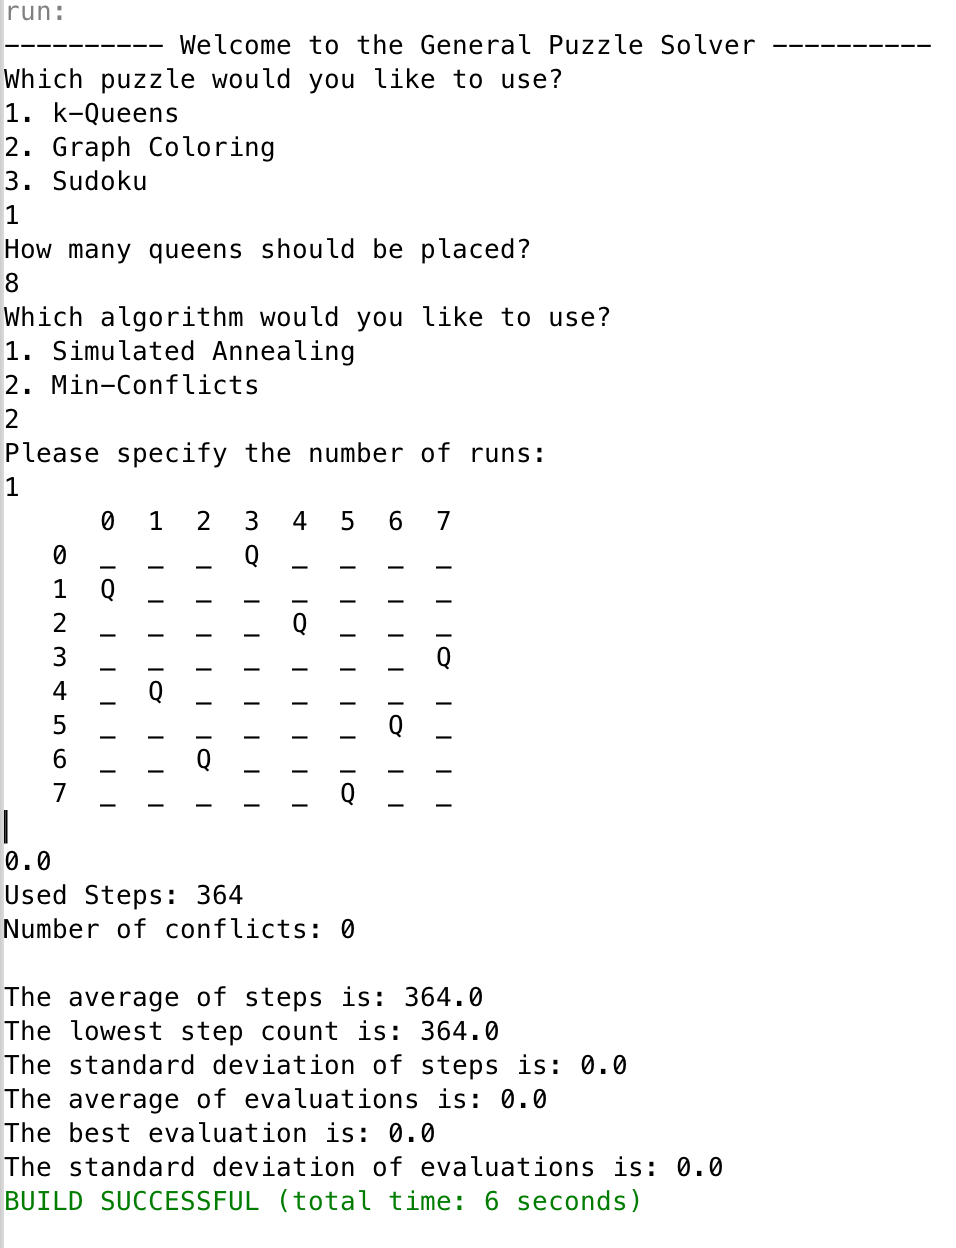
\includegraphics[width=1.0\linewidth]{graphics/queens-mc.png}
\caption{Solution of 8-Queens with min-conflicts.}\label{fig:queens-mc}
 \end{figure}

\pagebreak

\section{Second Puzzle: Graph Colouring}


\begin{table}[!htbp]
\caption{Statistics for the graph colouring puzzle.}
\begin{tabularx}{\textwidth}{l | X | X | X | X | X | X}
Combination & Evaluation  \newline Average & - \newline SD & - \newline Best & Steps \newline Average & - \newline SD & - \newline Lowest \\
\hline
Easy / SA & 0.0 & 0.0 & 0.0 & 68.1 & 25.10 & 40 \\
Medium / SA & 0.0 & 0.0 & 0.0 & 31.2 & 12.31 & 12  \\
Hard / SA & 0.0 & 0.0 & 0.0 & 607.94 & 48.16 & 520  \\
Easy / MC & 0.0 & 0.0 & 0.0 & 60.7 & 17.93 & 37  \\
Medium / MC & 0.0 & 0.0 & 0.0 & 33.2 & 9.12 & 12  \\
Hard / MC & 0.0 & 0.0 & 0.0 & 631.5 & 79.59 & 528   \\
\end{tabularx}
\end{table}


Both algorithms were able to solve the easy case variant of the graph colouring puzzle without problems. The results as shown by our application can be seen in \autoref{fig:graph-sa} for simulated annealing and \autoref{fig:graph-mc} for min-conflicts.

 \begin{figure}[!htbp]
 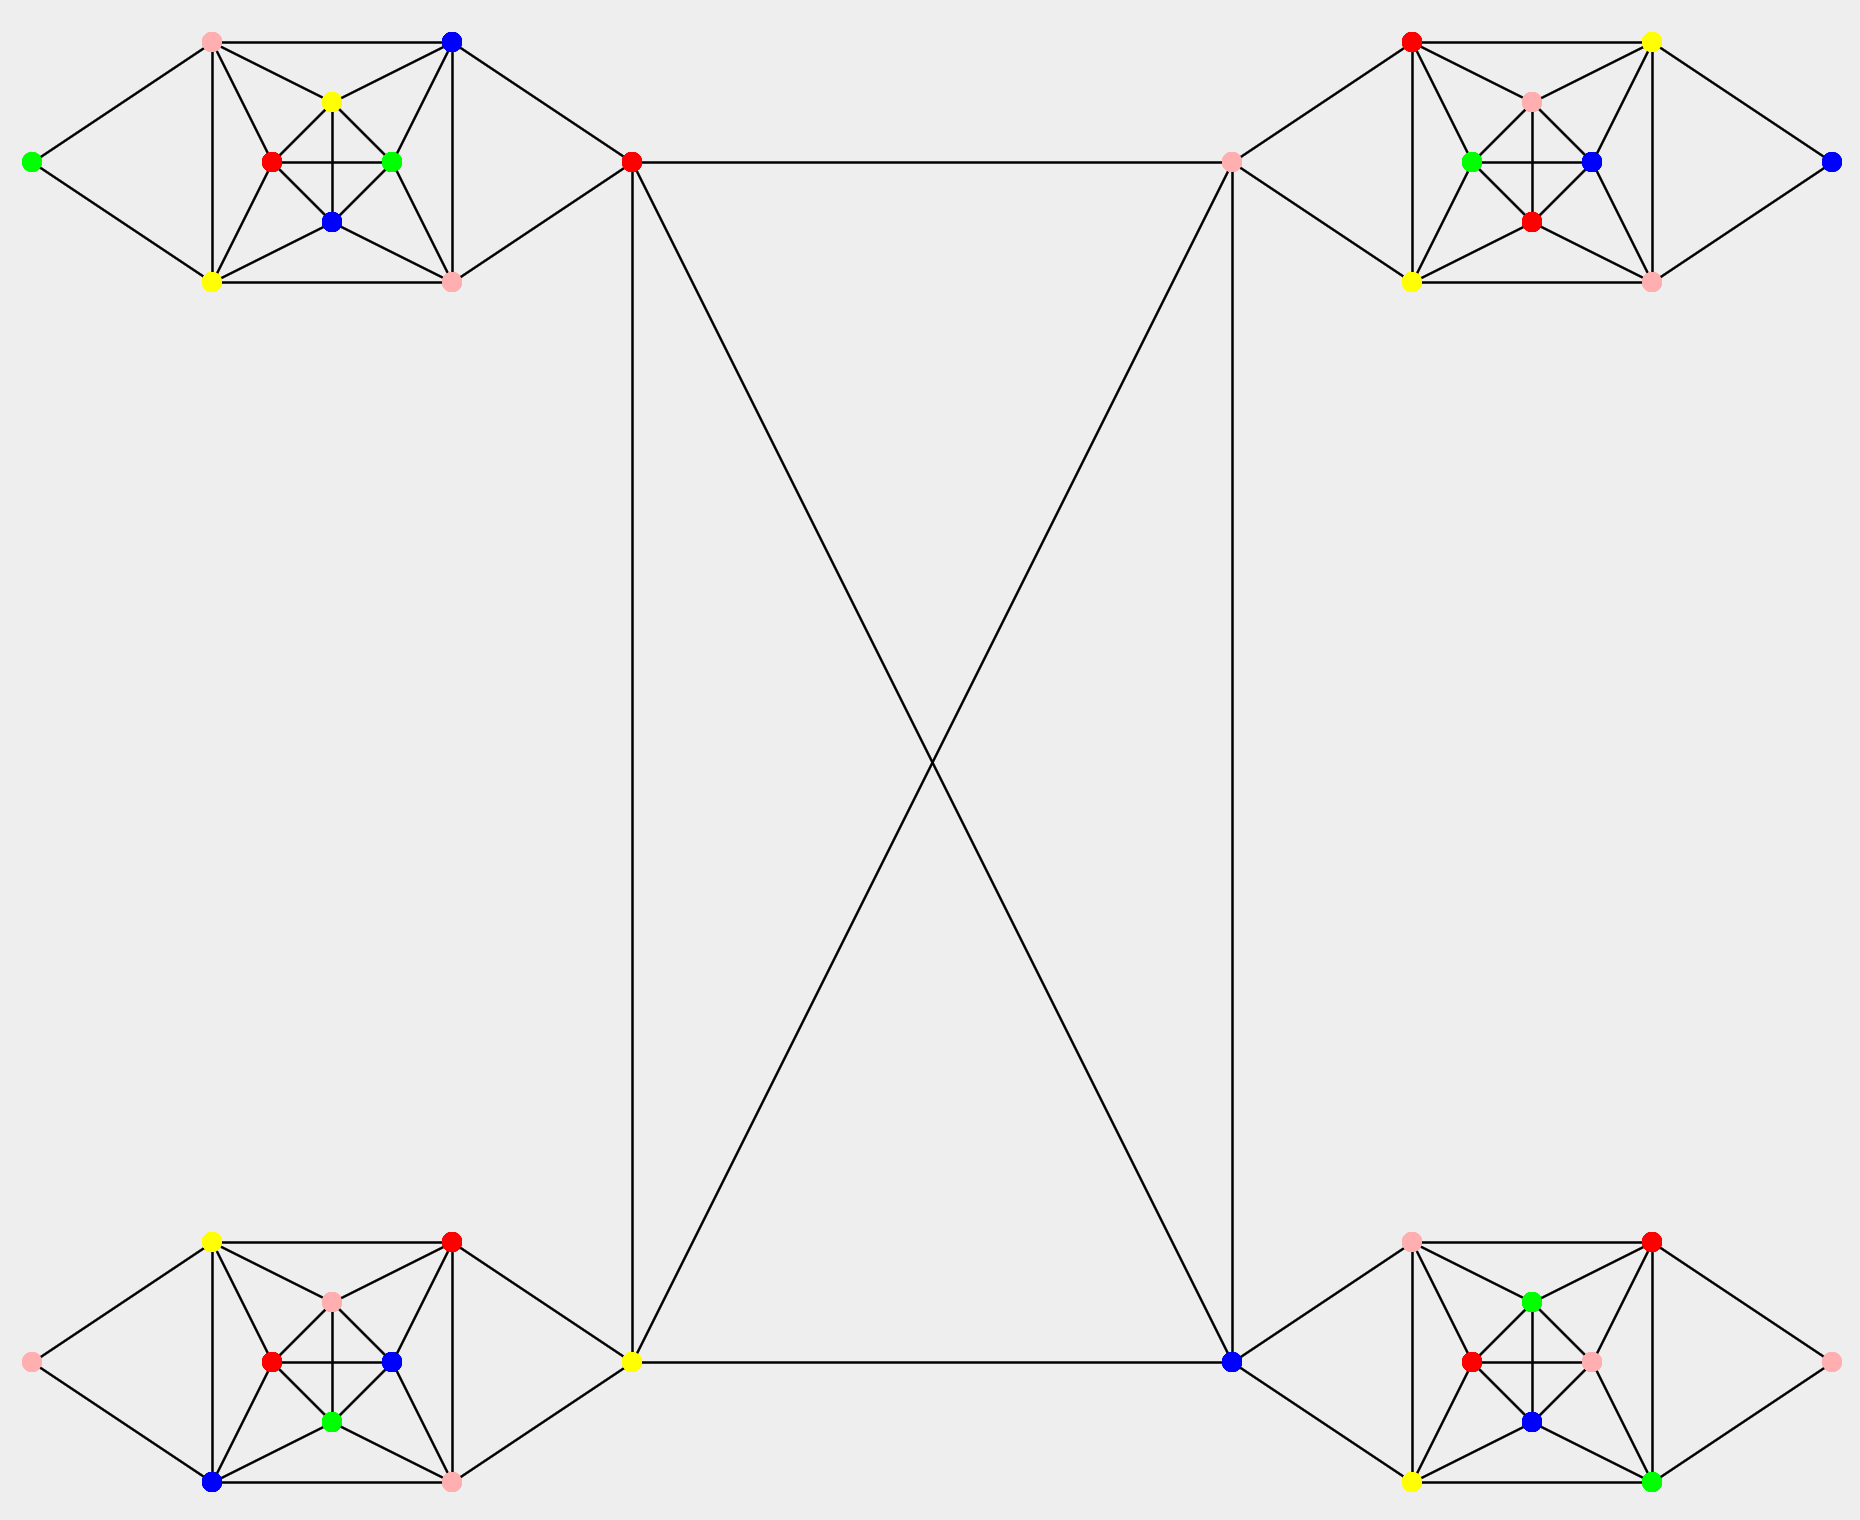
\includegraphics[width=1.0\linewidth]{graphics/graph-sa.png}
\caption{Solution of graph colouring with simulated annealing.}\label{fig:graph-sa}
 \end{figure}
 
  \begin{figure}[!htbp]
 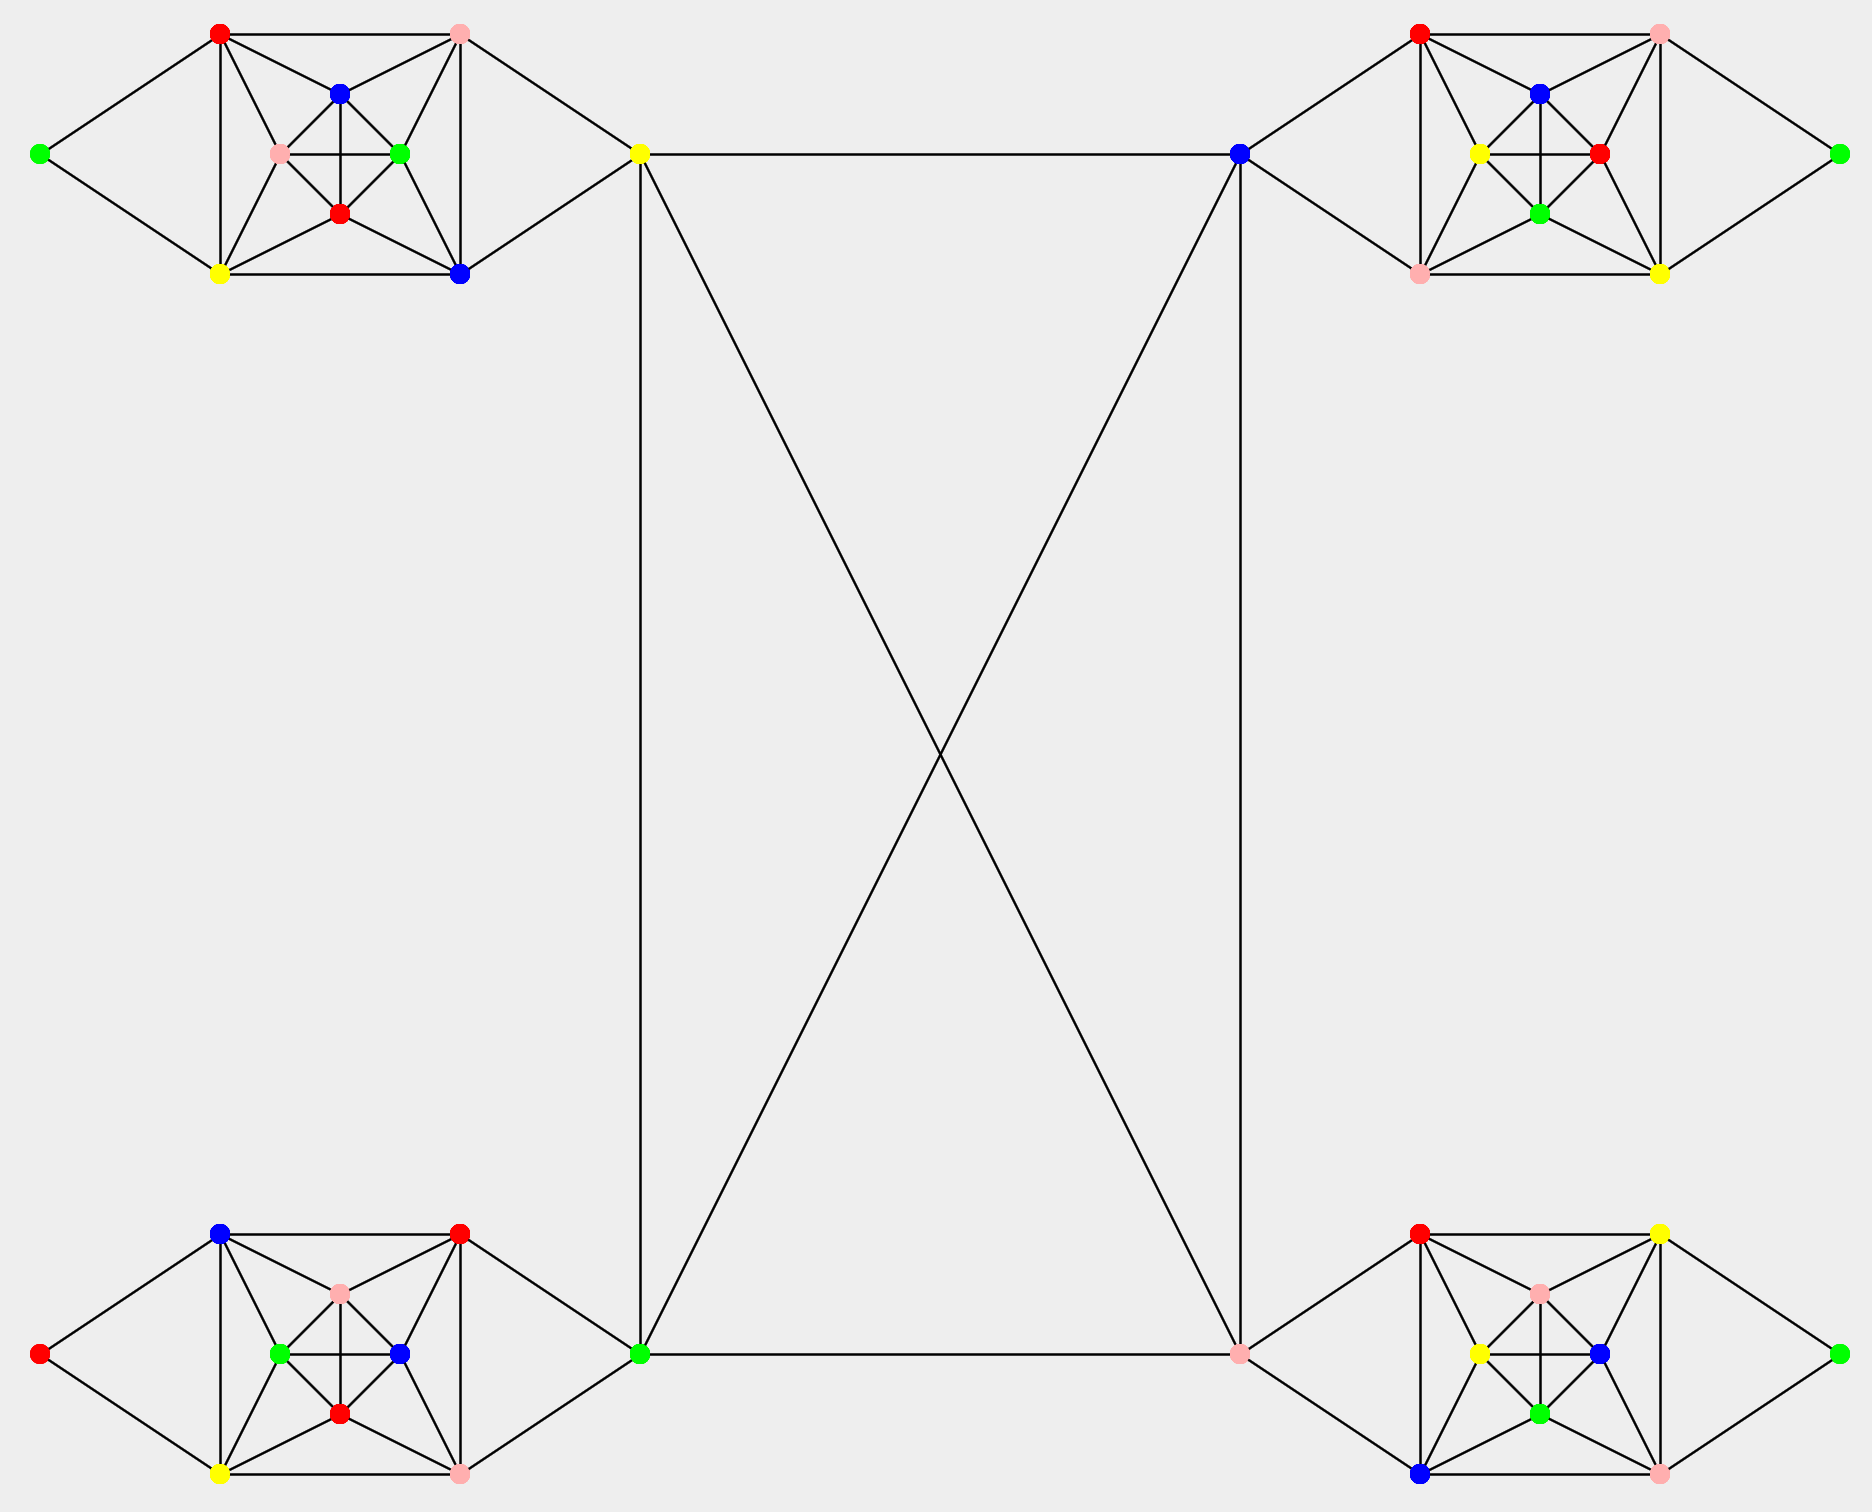
\includegraphics[width=1.0\linewidth]{graphics/graph-mc.png}
\caption{Solution of graph colouring with min-conflicts.}\label{fig:graph-mc}
 \end{figure}

\pagebreak

\section{Third Puzzle: Sudoku}

We chose to implement Sudoku as our third puzzle, which in hindsight wasn't a good decision because we weren't able to get the algorithms to solve it properly. With higher values for the maximum steps, it's possible to see, that the solutions seem to go in the right direction, but they somehow always get stuck at a local minimum of the count of the constraint violations.

In the \textit{SudokuPuzzleState} class we simply represent a state as a multidimensional array of integers. To not change initial values of the sudoku grid, we store a \textit{startingState} in the implementation of the state manager. Every position that has a value of 0 set in this starting state can be changed in other states.

Checking constraints of sudoku consists of going through all 81 numbers in the grid and comparing them to all the numbers in the same line, same column and same 3x3 block. Everytime a position with the same number is found, a new \textit{SudokuConflict} object is created by us. These consist of the position indices of the currently checked number and the position it was equal to. This should create a maximum of $81*24=1944$ conflicts if every number in the grid would be the same. As suggested in:

\begin{itemize}
\item \url{https://amoon.netfirms.com/Portfolio/Applied%20AI%20-%20Sudoku%20Solver.pdf},
\end{itemize}

we decided to apply higher values to conflicts with numbers from the starting state that can't be changed.

As with all the puzzles we implemented we create a double value to represent the evaluation by dividing the value of found conflicts by the maximum value for conflicts. This yields a value between 0.0 for a solution to the problem and 1.0 for the worst possible state.


\begin{table}[!htbp]
\caption{Statistics for the sudoku puzzle.}
\begin{tabularx}{\textwidth}{l | X | X | X | X | X | X}
Combination & Evaluation  \newline Average & - \newline SD & - \newline Best & Steps \newline Average & - \newline SD & - \newline Lowest \\
\hline
Easy / SA & 0.01219 & 0.00206 & 0.00720 & 10000.0 & 10000.0 & 0.0 \\
Medium / SA  & 0.01162 & 0.00272 & 0.00617 & 10000.0 & 10000.0 & 0.0  \\
Hard / SA  & 0.01203 & 0.00181 & 0.00925  & 10000.0 & 10000.0 & 0.0 \\
Easy / MC  & 0.06013 & 0.00682 & 0.05144  & 10000.0 & 10000.0 & 0.0 \\
Medium / MC & 0.03055 & 0.00639 & 0.01954 & 10000.0 & 10000.0 & 0.0  \\
Hard / MC & 0.04573 & 0.00691 & 0.03395  & 10000.0 & 10000.0 & 0.0  \\
\end{tabularx}
\end{table}


In \autoref{tab:start} and \autoref{tab:solution} you can see the starting state for the easy puzzle that was used and the solution to it. \autoref{fig:sudoku-sa} and \autoref{fig:sudoku-mc} show the results that simulated annealing and min-conflicts achieved after 10.000 steps.

\begin{table}[!htbp]
\caption{Starting state of the easy Sudoku puzzle.}
\label{tab:start}
\centering
\begin{tabularx}{5.8cm}{|c|c|c||c|c|c||c|c|c|}
\hline
0 & 0 & 6 & 2 & 4 & 0 & 0 & 0 & 0 \\
\hline
2 & 7 & 0 & 0 & 0 & 0 & 0 & 0 & 0 \\
\hline
8 & 4 & 0 & 0 & 7 & 5 & 0 & 3 & 0 \\
\hline
\hline
0 & 8 & 0 & 0 & 0 & 1 & 0 & 0 & 0 \\
\hline
0 & 1 & 0 & 4 & 0 & 9 & 0 & 5 & 0 \\
\hline
0 & 0 & 0 & 3 & 0 & 0 & 0 & 1 & 0 \\
\hline
\hline
0 & 3 & 0 & 1 & 9 & 0 & 0 & 4 & 8 \\
\hline
0 & 0 & 0 & 0 & 0 & 0 & 0 & 6 & 1 \\
\hline
0 & 0 & 0 & 0 & 5 & 8 & 7 & 0 & 0 \\
\hline
\end{tabularx}
\end{table}

\begin{table}[!htbp]
\caption{Hand-made solution of the easy Sudoku puzzle.}
\label{tab:solution}
\centering
\begin{tabularx}{5.8cm}{|c|c|c||c|c|c||c|c|c|}
\hline
9 & 5 & 6 & 2 & 4 & 3 & 1 & 8 & 7 \\
\hline
2 & 7 & 3 & 8 & 1 & 6 & 4 & 9 & 5 \\
\hline
8 & 4 & 1 & 9 & 7 & 5 & 6 & 3 & 2 \\
\hline
\hline
3 & 8 & 9 & 5 & 6 & 1 & 2 & 7 & 4 \\
\hline
7 & 1 & 2 & 4 & 8 & 9 & 3 & 5 & 6 \\
\hline
4 & 6 & 5 & 3 & 2 & 7 & 8 & 1 & 9 \\
\hline
\hline
6 & 3 & 7 & 1 & 9 & 2 & 5 & 4 & 8 \\
\hline
5 & 2 & 8 & 7 & 3 & 4 & 9 & 6 & 1 \\
\hline
1 & 9 & 4 & 6 & 5 & 8 & 7 & 2 & 3 \\
\hline
\end{tabularx}
\end{table}

 \begin{figure}[!htbp]
 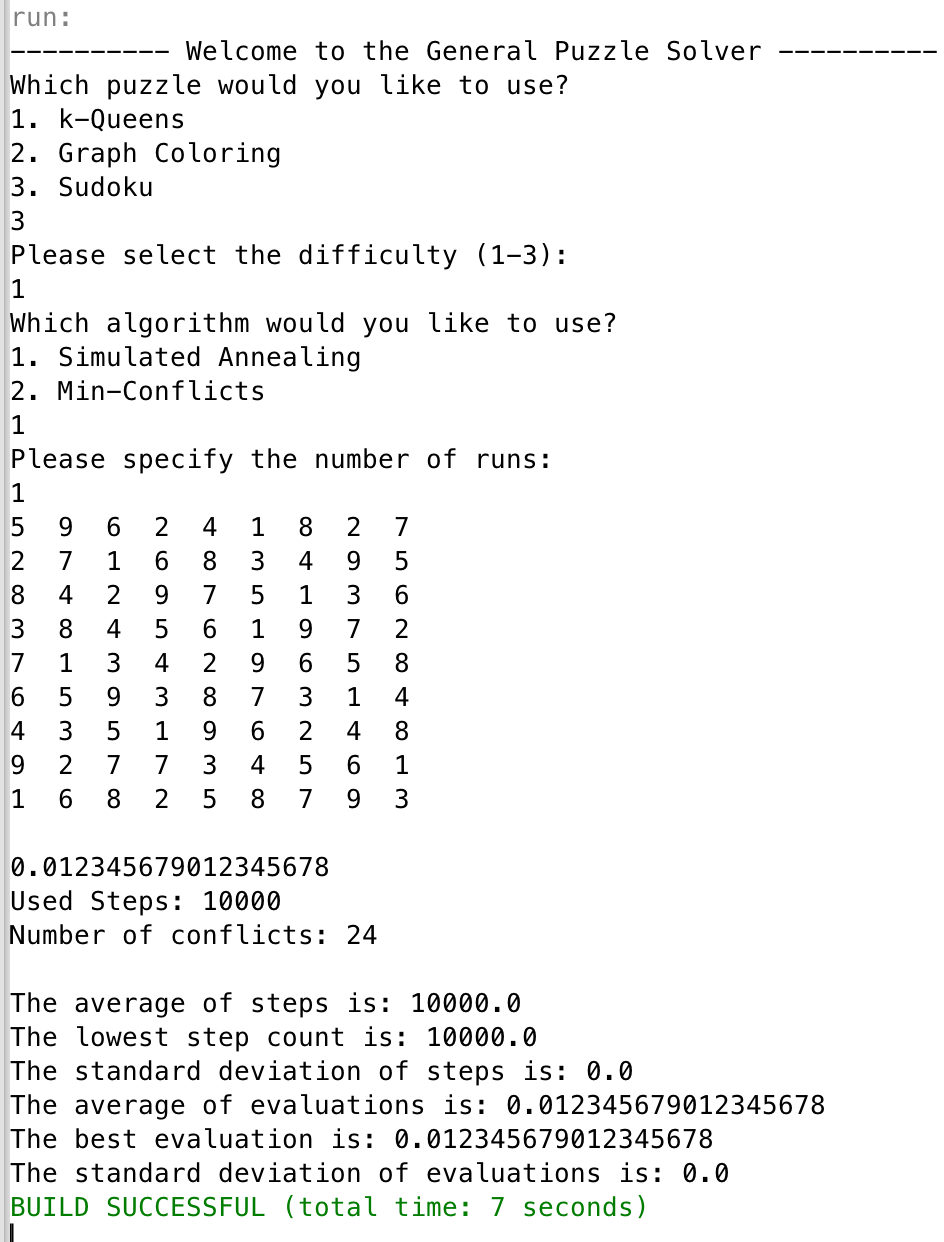
\includegraphics[width=1.0\linewidth]{graphics/sudoku-sa.png}
\caption{Best Solution of sudoku with simulated annealing.}\label{fig:sudoku-sa}
 \end{figure}
 
  \begin{figure}[!htbp]
 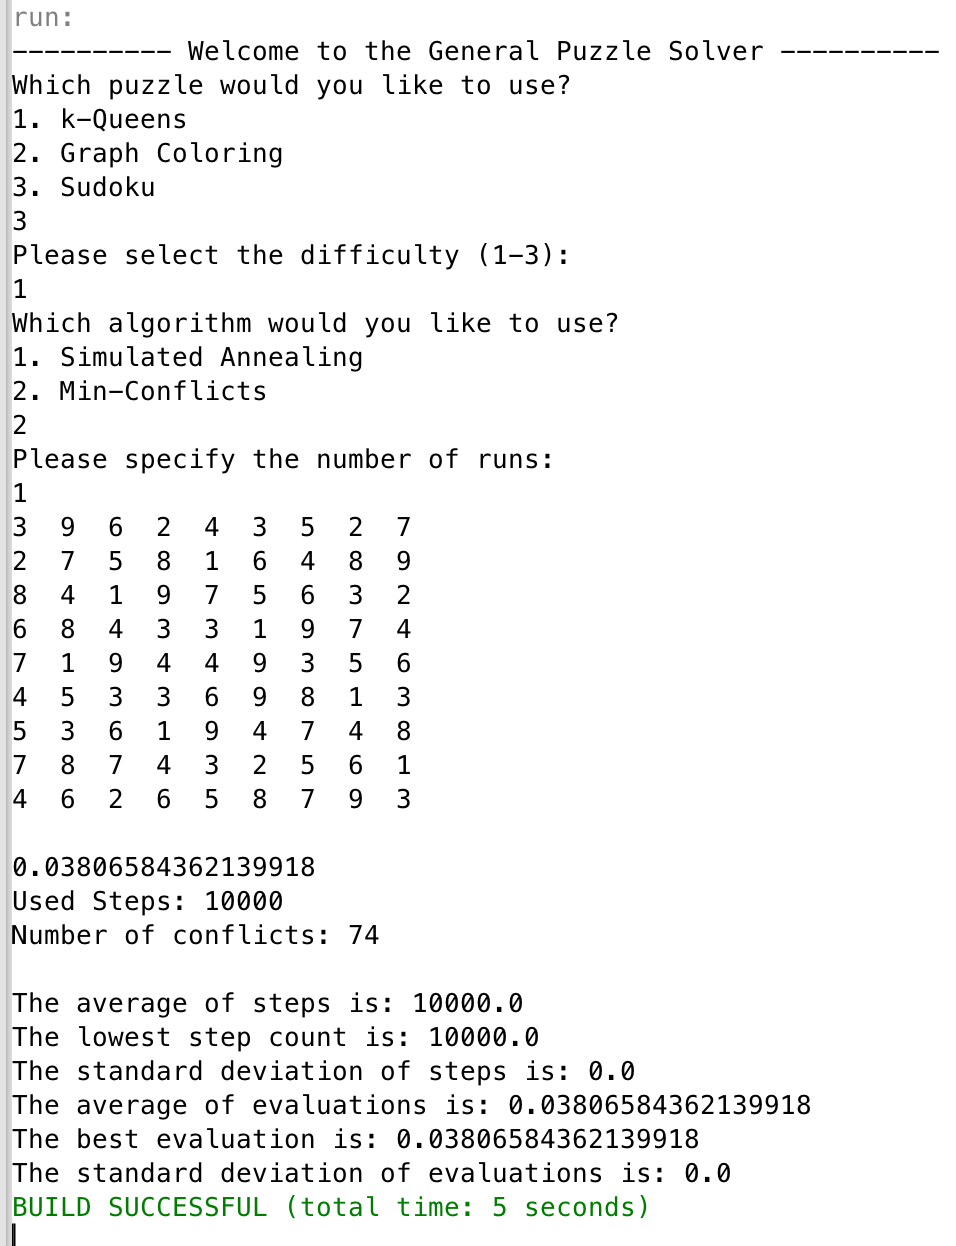
\includegraphics[width=1.0\linewidth]{graphics/sudoku-mc.png}
\caption{Best solution of sudoku with min-conflicts.}\label{fig:sudoku-mc}
 \end{figure}

\pagebreak


\end{document}
